% --- DVA218 lab 3 -------------------------
% | Information:                           |
% | If you only want to write the text and |
% | don't want to change settings place    |
% | go to the row that have the comment    |
% | -- Start writing here---               |
% ------------------------------------------

% ------------- START SETTINGS -------------------------------
\documentclass[conference]{IEEEtran}
\usepackage{blindtext, graphicx}

\ifCLASSINFOpdf
\else
\fi

% A couple of useful packages
\usepackage[table]{xcolor}
\usepackage{listings}
\usepackage{color}
\usepackage{amsmath}
\usepackage{subfiles}
\usepackage{verbatim}
 
 % Programming color don't touch without permissions.
\definecolor{codegreen}{rgb}{0,0.6,0}
\definecolor{codeblue}{HTML}{0073e6}
\definecolor{codegray}{rgb}{0.4,0.4,0.4}
\definecolor{codeblac}{rgb}{0.9,0.9,0.9}
\definecolor{commentgray}{rgb}{0.7,0.7,0.7}
\definecolor{codepurple}{rgb}{0.58,0,0.82}
\definecolor{stringblue}{HTML}{0073e6}
\definecolor{stringpurple}{HTML}{ff99ff}
\definecolor{stringgray}{rgb}{0.6,0.6,0.6}
\definecolor{backcolour}{rgb}{1,1,1}
 
\lstdefinestyle{mystyle}{
    backgroundcolor=\color{backcolour},   
    commentstyle=\color{commentgray},
    keywordstyle=\color{codeblac},
    numberstyle=\tiny\color{codegray},
    stringstyle=\color{stringgray},
    basicstyle=\footnotesize,
    breakatwhitespace=false,         
    breaklines=true,                 
    captionpos=b,                    
    keepspaces=true,                 
    numbers=left,                    
    numbersep=5pt,                  
    showspaces=false,                
    showstringspaces=false,
    showtabs=false,                  
    tabsize=2
}
 
\lstset{style=mystyle}
\lstset{language=c} % C is the default language in listings.

\usepackage{mdwmath}
% --- packages for state machine ----
\usepackage{tikz}
\usetikzlibrary{arrows,automata}
% --- end state -------------------------

\begin{document}
\title{DVA218 - Assignment 3a and 3b}
\author{\IEEEauthorblockN{Hampus Baaz}
\and
\IEEEauthorblockN{Wicktor L{\"o}w}
\and
\IEEEauthorblockN{Magnus S{\"o}rensen}}
% make the title area
\maketitle

${}$\hspace{5em}

%\IEEEpeerreviewmaketitle

%\vspace{10 mm}

% --- END SETTINGS --------------------------------------------

%  |~~~Start writing here----------------
%  |--->

\section{Introduction}
This is the first part of two in an assignment with the goal to create a reliable and efficient transport protocol on top of UDP. This first part contains state-machines for the different modules we will be implementing later in the code. There are three different modules, a connection with a three-way handshake, a sliding window protocol with selective acknowledgements and a teardown protocol. Each module will be described with two state machines, one for the sender (client) and one for the receiver (server).

\section{State machines}
Below we have six different Moore-styled state machines with figures and text describing how our modules will be implemented.

\subsection{Three-way handshake - Client}
  
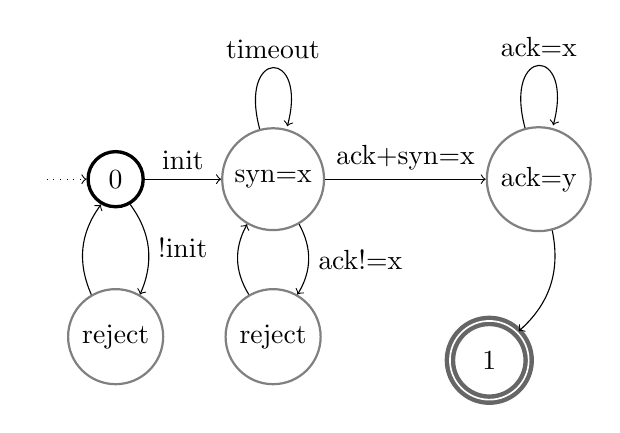
\begin{tikzpicture}
[
init/.style={circle, draw=black!100, very thick, minimum size=7mm,node distance=2cm},
state_split/.style={circle, draw=gray!100, thick, minimum size=7mm,node distance=2cm},
state/.style={circle, draw=gray!100, thick, minimum size=7mm,node distance=2cm},
final/.style={circle, double, draw=black!60,  ultra thick, minimum size=10mm,node distance=23mm}
]
%Nodes
\node[init]             (start)                         {0};
\node                   (em)        [left of=start]     {};
\node[state_split]      (reject)    [below of=start]    {reject};
\node[state_split]      (synx)      [right of=start]    {syn=x\nodepart{lower} 2};
\node[state]      (end)       [right of=synx, right=7mm]     {ack=y};
\node[state_split]      (rejected)  [below of=synx]     {reject\nodepart{lower}3};
\node[final]            (end2)      [below of=end, left=1mm]      {1};


%Lines
\draw[dotted, ->] (em.east) -- (start.west);
\path[->] 
(start)   edge [bend left]        node[right]     {!init}     (reject)
(reject)  edge [bend left]        node[left]      {}         (start)
(start)   edge                    node[above]     {init}      (synx)
(synx)    edge [bend left]        node[right]     {ack!=x}      (rejected)
(rejected) edge [bend left]       node[left]      {}        (synx)
(synx)    edge                    node[above]     {ack+syn=x}     (end)
(end)     edge [loop above]       node            {ack=x}     (end)
(synx)  edge    [loop above]      node            {timeout}    (synx)
(end)   edge    [bend left]       node            {}         (end2);
\end{tikzpicture}

\\
The client start out by sending a synchronisation package (sync) to the server, this package contains information for the sliding window protocol, e.g. window size and number of packages it wants to send. After sending this sync it will wait to receive an acknowledgement (ACK) from the server. If it receives a wrong ACK it will proceed to send a reject back to the server then send a new sync package, if it takes to long time and goes to timeout it will also resend the sync. When it finally receives the right ACK it will establish a connection to the server. In the final stage, the client will discard any ACK:s that might have fallen behind and come in late.  
\subsection{Three-way handshake - Server}
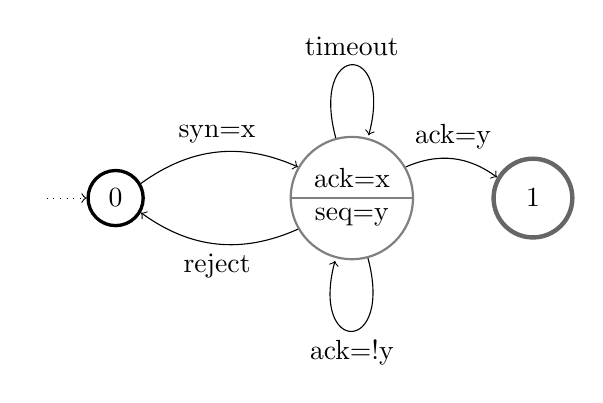
\begin{tikzpicture}
[
init/.style={circle, draw=black!100, very thick, minimum size=7mm,node distance=2cm},
state_split/.style={circle split, draw=gray!100, thick, minimum size=7mm,node distance=3cm},
state/.style={circle, draw=gray!100, thick, minimum size=7mm,node distance=2cm},
final/.style={circle, draw=black!60,  ultra thick, minimum size=10mm,node distance=23mm}
]
%Nodes
\node[init]     (start)                         {0};
\node           (init)        [left of=start]     {};
\node[state_split]    (synx)      [right of=start]    {ack=x\nodepart{lower}seq=y};
\node[final]    (end)       [right of=synx]     {1};



%Lines
%\draw[->] (start.east) -- (synx.west);
%\draw[->] (synx.east) -- (end.west);
%\path[->] (start)  edge [loop above] node {a} (start); 
\draw[dotted, ->] (init.east) -- (start.west);
\path[->] 
          (start)   edge[bend left]     node[above]     {syn=x}     (synx)
          (synx)    edge[bend left]     node[below]     {reject}    (start)
          (synx)    edge[loop above]    node            {timeout}   (synx)
          (synx)    edge[loop below]    node            {ack=!y}     (synx)
          (synx)    edge[bend left]     node[above]     {ack=y}     (end);

\end{tikzpicture}
\\
The server will be idle, waiting for any incoming connections. When it receives the sync from the client it will send and ACK on this and a sequence number (seq). After sending this it will wait for an ACK for the seq or after a timeout resend the same information. If it by any change gets the wrong ACK back it will again resend the ACK and seq. When it receive and ACK on the seq it will establish connection with the client and be ready to receive packages.
\subsection{Teardown - Initializing host}
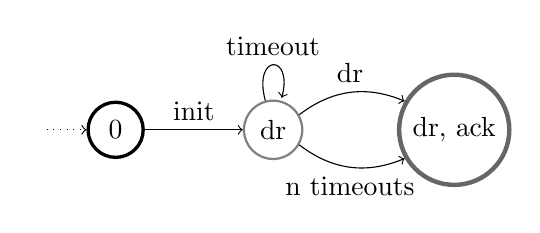
\begin{tikzpicture}
[
init/.style={circle, draw=black!100, very thick, minimum size=7mm,node distance=2cm},
state_split/.style={circle split, draw=gray!100, thick, minimum size=7mm,node distance=2cm},
state/.style={circle, draw=gray!100, thick, minimum size=7mm,node distance=2cm},
final/.style={circle, draw=black!60,  ultra thick, minimum size=10mm,node distance=23mm}
]
%Nodes
\node[init]         (start)                         {0};
\node               (em)        [left of=start]     {};
\node[state]        (send_dr)   [right of=start]    {dr};
\node[final]        (dc_ack)    [right of=send_dr]  {dr, ack};


%Lines
%\draw[->] (start.east) -- (synx.west);
%\draw[->] (synx.east) -- (end.west);
%\path[->] (start)  edge [loop above] node {a} (start); 
\draw[dotted, ->] (em.east) -- (start.west);
\path[->] 
(start)   edge                   node [above]   {init}      (send_dr)
(send_dr) edge [bend left]       node [above]   {dr}        (dc_ack)
(send_dr) edge [bend right]      node [below]   {n timeouts}  (dc_ack)
(send_dr) edge [loop above]      node           {timeout}   (send_dr);
\end{tikzpicture}

\\
Either the server or client should be able to initialize the teardown protocol.
\\
It do so by sending a disconnection request (dr) to the target host and at the same time start a timer. If it receives an ACK that the other host is disconnecting or after n timeout it will proceed to disconnect and send an ACK on this. 
\subsection{Teardown - Target host}
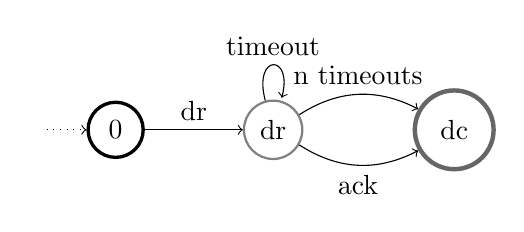
\begin{tikzpicture}
[
init/.style={circle, draw=black!100, very thick, minimum size=7mm,node distance=2cm},
state_split/.style={circle split, draw=gray!100, thick, minimum size=7mm,node distance=2cm},
state/.style={circle, draw=gray!100, thick, minimum size=7mm,node distance=2cm},
final/.style={circle, draw=black!60,  ultra thick, minimum size=10mm,node distance=23mm}
]
%Nodes
\node[init]         (start)                         {0};
\node               (em)        [left of=start]     {};
\node[state]        (send_dr)   [right of=start]    {dr};
\node[final]        (dc_ack)    [right of=send_dr]  {dc};


%Lines
%\draw[->] (start.east) -- (synx.west);
%\draw[->] (synx.east) -- (end.west);
%\path[->] (start)  edge [loop above] node {a} (start); 
\draw[dotted, ->] (em.east) -- (start.west);
\path[->] 
(start)   edge                   node [above]   {dr}    (send_dr)
(send_dr) edge [bend left]       node [above]   {n timeouts} (dc_ack)
(send_dr) edge [bend right]      node [below]   {ack}     (dc_ack)
(send_dr) edge [loop above]      node           {timeout}   (send_dr);
\end{tikzpicture}
\\
Here we have a problem, if all the disconnection requests sent from the initializing host get lost, the host will never know that it should disconnect, and that is something we just have to accept.
\\
However when the host receives the dr it will send a dr back and wait for an ACK, when it receives an ACK back or after n timeouts it will proceed to disconnect.
\subsection{Sliding window sender state machine}
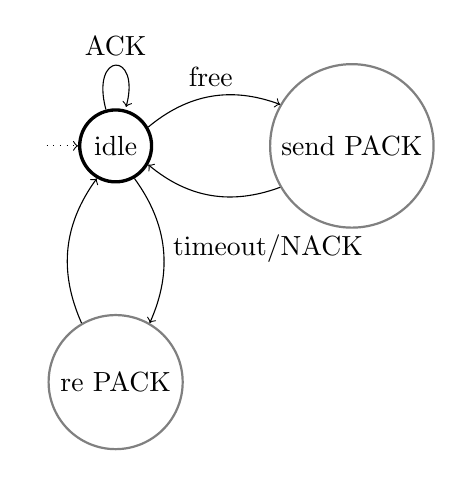
\begin{tikzpicture}
[
init/.style={circle, draw=black!100, very thick, minimum size=7mm,node distance=1cm},
state_split/.style={circle split, draw=gray!100, thick, minimum size=7mm,node distance=3cm},
state/.style={circle, draw=gray!100, thick, minimum size=7mm,node distance=3cm},
final/.style={circle, draw=black!60,  ultra thick, minimum size=10mm,node distance=23mm}
]
%Nodes
\node[init]     (start)                         {idle};
\node           (init)          [left of=start]     {};
\node[state]    (sack)          [right of=start]    {send PACK};
\node[state]    (reack)         [below of=start]    {re PACK};



%Lines
%\draw[->] (start.east) -- (synx.west);
%\draw[->] (synx.east) -- (end.west);
%\path[->] (start)  edge [loop above] node {a} (start); 
\draw[dotted, ->] (init.east) -- (start.west);
\path[->] 
          
(start) edge[bend left]         node[above]             {free}      (sack)
(sack)  edge[bend left]         node[below]             {}          (start)
(start) edge[bend left]         node[right]             {timeout/NACK} (reack)
(reack) edge[bend left]         node[left]              {}          (start)
(start) edge[loop above]        node[above]             {ACK}       (start);

\end{tikzpicture}
\\For the sliding windows itself it starts of in the idle state. If there is free space in the window, packages will be sent. If and when the ACK comes back nothing really happens in the case of input and output. Though the ack will be stored together with the sent message so knowing which packages the program knows has been received by the receiver side. There will also be movement in the windows size and there could be the possibility to receive a NACK to resend a package but that will probably not be used. If a package is lost the receiver will still ACK packages after the lost one so only the lost package will be really affected. If no ACK (selective) arrives on a sent package the specific package will be resent after that package is timed out.
\subsection{Sliding window receiver state machine}
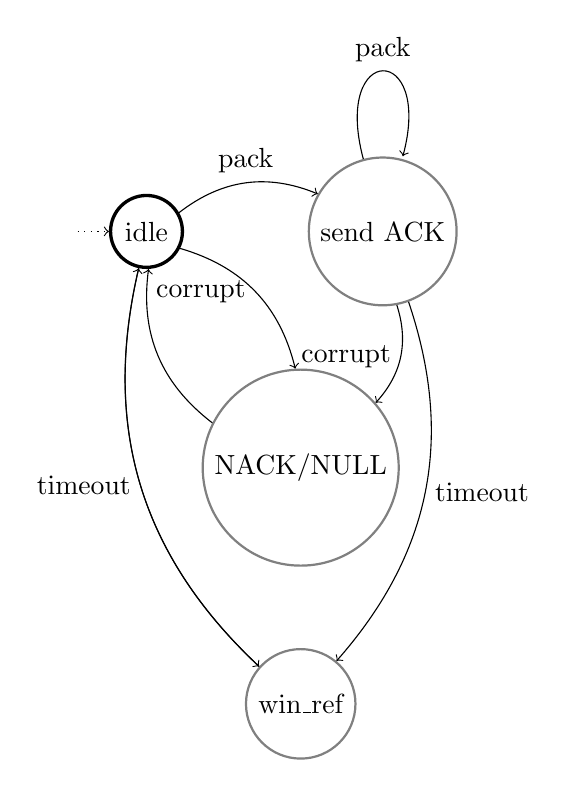
\begin{tikzpicture}
[
init/.style={circle, draw=black!100, very thick, minimum size=7mm,node distance=1cm},
state_split/.style={circle split, draw=gray!100, thick, minimum size=7mm,node distance=3cm,inner sep=0},
state/.style={circle, draw=gray!100, thick, minimum size=7mm,node distance=3cm},
final/.style={circle, draw=black!60,  ultra thick, minimum size=10mm,node distance=23mm}
]
%Nodes
\node[init]     (start)                         {idle};
\node           (init)          [left of=start]     {};
\node[state]    (ack)          [right of=start]    {send ACK};
\node[state]    (nack)         [below of=start, right=7mm]    {NACK/NULL};
%\node[state]    (wref)         [below of=nack]    {win_ref};
\node[state]    (wref)          [below of=nack]      {win\_ref};

%Lines
%\draw[->] (start.east) -- (synx.west);
%\draw[->] (synx.east) -- (end.west);
%\path[->] (start)  edge [loop above] node {a} (start); 
\draw[dotted, ->] (init.east) -- (start.west);
\path[->] 

(start) edge[bend left]                   node[above]             {pack}      (ack)
(start) edge [bend right]        node[left]             {timeout}   (wref)
(ack)   edge[loop above]        node[above]             {pack}      (ack)
(ack)   edge [bend left]        node[left]              {corrupt}   (nack)
(start) edge [bend left]        node[left]              {corrupt}   (nack)
(nack)  edge [bend left]        node                    {}          (start)
(ack)   edge [bend left]        node[right]             {timeout}   (wref)
(wref)  edge [bend left]        node                    {}          (start);





\end{tikzpicture}
\\The receiver have two main states, one idle state with no output and another state that sends ACK. When a package is received it goes to the other state that sends back an ACK for that package. This state will be rerun every time a new good package is arriving and ACK those packages. If a corrupt package is received there was a idea to nack that one but with corrupted information about the package itself that will not be possible. So if a corrupt package is received it will just be ignored and let the server timeout that package and resend it. It would in this case not need its own state so the \textbf{NACK/NULL} would not exist and the arrows would just go to idle but the state is there for illustration. If by some reason the receiver buffer was full when the last ACK was sent the server will not send any new packages. So if no packages has been received for a while a window refresh will be sent back to the sender to make sure the sender knows that there is free space. 
\section{How to download the program}
Our implementation of the program can be downloaded from git hub using the following command on a machine that have the git package installed.
\begin{lstlisting}
 $ git clone https://github.com/byteofsoren/DVA218-lab3.git
\end{lstlisting}

\section{How to execute the program}
Before executing the program its need to be compiled using the make program.
\begin{lstlisting}
 $ cd DVA218-lab3
 $ make all
\end{lstlisting}

There is also a CMakeLists.txt if that is preferred to compile with. It is for building with CLion IDE but should be able to compile in regular terminal as well.


This implementation of the program uses command line argument to define if the program is going to be a server or a client. If no argument is passed the program is going to be executed as a server. Like this.

\begin{lstlisting}
  $ ./prog.out
\end{lstlisting}

To execute the program as a client simply specify what address you want to send to.
\begin{lstlisting}
  $ ./prog.out localhost
\end{lstlisting}

or for example using a IP number. 
\begin{lstlisting}
  $ ./prog.out 130.243.87.87
\end{lstlisting}
 
If the project was compiled with CMake the executable is called little bit different but the rest is the same. The executeble will also in lie in a sub-folder of the project called cmake-build-debug/
\begin{lstlisting}
  $ ./dva218-lab3
\end{lstlisting}


After the initial handshake we are asked to type message and finish by pressing enter. Now the internal logic takes over and sends the message over socket to the other computer. When it was successfully delivered to the server the program end.

\section{Errors}\label{subsec:errors}
\subsection{Check sum}\label{subsec:csum}
Before a package is sent to a receiver the program calculates the check sum by  first setting the packages check sum to zero and then serialising the package to a buffer array. Then the buffer array is then iterated over and byte by byte to sum up to a value that is then stored in the packages check sum. The receiver does almost the same thing as the sender. It stores the check sum in a temporary variable and set the package check to zero and then do the serialisation mentioned above. If the result of the check sum is equal to the temporary variable then the package is considered unchanged.
\subsection{Error Generation}\label{subsec:errGen}
The error simulation in this program is done by a function that is named \textbf{errorGenerator}. This generator works by percentage of chance to get a error and multiple error can happen on the same package. In our case we can generate the following type of error to a package. 
\begin{enumerate}
    \item Check sum error
    \item Package got out of order
\end{enumerate}
The check sum error is just a random new check sum that is applied to the package. The out of order part of the error generator is using a array as a jail that can randomly store the package for a short period of time. By using that solution the package can arrive to the receiver out of order or even be double written on the socket connection, simulating that a package has taken a longer route and arrives delayed. 

\subsection{Error Detection}\label{subsec:errDet}
The error detection relies on the previously mentioned method in the subsection Check sum \ref{subsec:csum}. If the package is corrupt the read function return a negative answer and the package is considered lost.


\section{Receiver}\label{sec:receiver}
To split the problem there is now a receiver and a sender since both server and clients do have receiving and sending sections.
The receiver have a simple job of handling faulty packets. If something is wrong it is found in Error Detection which is in \textbf{ingsoc\_readMessage} and the returns from that function needs to be 0 for a OK packet. If read find a problem there is two ways it is handled. Some places the toRead is set to init (0 and false on everything) but most often all code about the read message is skipped and the result is the same as a timeout. This is resend the last message and wait for the correct package again.\\
For example from \textbf{server.c} in the three way handshake if the \textbf{ingsoc\_readMessage} returns -1 (which it does with checksum or ID faults) the read is zeroed to reach the else statement. This in turn have the same outcome as a message with no ACK or a timeout (in this specific case, most often a timeout). Increasing the counter and running the specific part of three-way again and if it has tried enough times it gives up.
\lstinputlisting[firstline=186, lastline=202, frame=single]{server.c}

\section{Sender}\label{sec:sender}
The sender really doesn't know that anything is wrong. If the sent packet had anything that made the receiver dismiss it the sender will just timeout and resend when it doesn't receive an ACK on that package. In some cases like the one in receiver above where it resend their package the sender will have a package it didn't expect (in three-way and teardown). This in turn will make the sender to a receiver and it will do a resend of its package and wait for a return. Since the package that is resent from both sides is the package the other side expect it moves on very quickly moving to sliding window.\\
Even though this example is for three-way handshake the same principle remain for all other parts of the code except what message is resent and when. Sliding window for example only do resend on timeout and the server (receiver) just doesn't send ACK on faulty packages and really old packages. 

\section{Differences between theoretical and implementation}\label{sec:changes}
There has been some minor changes in the concept from when we first created our state machines to when our solution was done. 
\subsection{Three-way Handshake}\label{subsec:TWshake}
There wasn't really any notable changes to the three-way handshake in either the server or the client part. The small difference was to not implement any reject and that meant that client became easier. This meant that fault in threeway is only handled by timeout. 

\subsection{Sliding Window Protocol}\label{subsec:SWP}
We did have vague plans to use negative acknowledgements (NACK) in our sliding window protocol but we ended up not using this solution. Instead the sender puts a timer on each package it sends and if it doesn't receive an ACK in this period of time for that package it will timeout and resend the package.\\
On the receiver side of the sliding window we first wanted to have two different scenarios, one if we receive a corrupt package and one if we don't receive any packages. The scenario where we don't receive a package that we expect the plan was to wait for a timeout and then just assume it is either done or the connection is lost so we would disconnect. Now however we came to the conclusion that it was a bad idea to give up so easy, so instead it is handled from the sender side to make sure the packages is sent when something is corrupt or get lost, the receiver just keep waiting for packages and then finally a disconnection request when all the packages is sent.

\subsection{Teardown}\label{subsec:tear_down}
We first intended the teardown to be implemented so that either side could initialize the disconnect protocol, but we it ended up always being the sender that sends the disconnection request when it is done sending packages. 


\lstinputlisting[language= , frame=single]{server.c}

\end{document}